\documentclass[11pt]{article}

% --- Packages ---
\usepackage[utf8]{inputenc}
\usepackage[T1]{fontenc}
\usepackage{amsmath,amssymb,amsfonts}
\usepackage{graphicx}
\usepackage{booktabs}
\usepackage{hyperref}
\usepackage{xcolor}
\usepackage{listings}
\usepackage{algorithm}
\usepackage{algpseudocode}
\usepackage[margin=1in]{geometry}
\usepackage{caption}
\usepackage{subcaption}
\usepackage{enumitem}
\usepackage{natbib}
\usepackage{multirow}
\usepackage{array}
\usepackage{tabularx}
\usepackage{float}

% --- Hyperref settings ---
\hypersetup{
    colorlinks=true,
    linkcolor=blue!60!black,
    citecolor=blue!60!black,
    urlcolor=blue!60!black,
}

% --- Code listing style ---
\definecolor{codebg}{RGB}{245,245,245}
\definecolor{codegreen}{RGB}{40,160,40}
\definecolor{codegray}{RGB}{128,128,128}
\definecolor{codepurple}{RGB}{160,32,240}

\lstdefinestyle{python}{
    backgroundcolor=\color{codebg},
    basicstyle=\ttfamily\small,
    breaklines=true,
    captionpos=b,
    commentstyle=\color{codegreen},
    keywordstyle=\color{codepurple}\bfseries,
    stringstyle=\color{orange},
    numberstyle=\tiny\color{codegray},
    numbers=left,
    numbersep=5pt,
    frame=single,
    framesep=5pt,
    language=Python,
    showstringspaces=false,
    tabsize=4,
    morekeywords={self,True,False,None,as,with,yield,mx,nn,mlxsnn},
}

\lstset{style=python}

% --- Title ---
\title{\textbf{Comprehensive Benchmarking of Spiking Neural Networks\\on Apple Silicon: mlx-snn v0.4}}

\author{
    Jiahao Qin \\
    \texttt{Jiahao.qin19@gmail.com}
}

\date{}

\begin{document}

\maketitle

% ===================================================================
% ABSTRACT
% ===================================================================
\begin{abstract}
We present a comprehensive benchmarking study of spiking neural network (SNN) training on Apple Silicon using mlx-snn v0.4, the first SNN library built natively on Apple's MLX framework. Since the initial release~\citep{qin2026mlxsnn}, mlx-snn has been extended with recurrent neuron models (RLeaky, RSynaptic), learnable decay and threshold parameters, five surrogate gradient functions (fast sigmoid, arctan, sigmoid, triangular tent, straight-through), three classification loss functions, and bidirectional interoperability with the Neuromorphic Intermediate Representation (NIR) standard. We conduct a systematic five-experiment benchmark study on MNIST digit classification, evaluating the effects of neuron type, learnable parameters, surrogate gradient function, loss function, and spike encoding strategy, each averaged over five random seeds. We provide the first cross-framework comparison between mlx-snn on an Apple M3 Max and snnTorch on an NVIDIA V100, revealing that mlx-snn achieves $3.7\times$ faster training per epoch while maintaining competitive classification accuracy ($96.3\%$ vs.\ $97.4\%$ for the baseline LIF configuration). Our analysis identifies critical sensitivity of recurrent neurons to the initialization of the recurrent weight $V$, demonstrates that the triangular tent surrogate gradient significantly outperforms snnTorch's sign-flipping variant, and provides practical guidelines for SNN hyperparameter selection on Apple Silicon. All code, configurations, and analysis scripts are publicly available.
\end{abstract}

\noindent\textbf{Project:} \url{https://github.com/D-ST-Sword/mlx-snn} \quad \textbf{PyPI:} \texttt{pip install mlx-snn}

% ===================================================================
% 1. INTRODUCTION
% ===================================================================
\section{Introduction}

Spiking neural networks (SNNs), often called the ``third generation'' of neural networks~\citep{maass1997networks}, process information through discrete spike events rather than continuous-valued activations. This biologically inspired computation paradigm offers several distinctive advantages: temporal coding of information that naturally captures time-varying patterns, event-driven processing with potential for significant energy savings, and direct compatibility with emerging neuromorphic hardware platforms~\citep{davies2018loihi, roy2019towards}. The development of surrogate gradient methods~\citep{neftci2019surrogate, zenke2021remarkable} has enabled SNNs to be trained with standard gradient descent, bringing modern deep learning optimization techniques to the spiking domain and steadily narrowing the accuracy gap with conventional artificial neural networks.

A growing ecosystem of software frameworks supports SNN research. snnTorch~\citep{eshraghian2023training} provides PyTorch-based neuron models with an intuitive, tutorial-rich interface. Norse~\citep{pehle2021norse} emphasizes functional programming and biological plausibility. SpikingJelly~\citep{fang2023spikingjelly} offers high-performance CUDA kernels for large-scale training. Lava~\citep{lava2021} targets Intel's Loihi neuromorphic processor. However, all of these frameworks are built on PyTorch~\citep{paszke2019pytorch} or custom backends, binding SNN research to the NVIDIA CUDA ecosystem. Researchers using Apple Silicon hardware --- which has seen rapid adoption in the machine learning community due to its unified memory architecture and competitive performance-per-watt --- have lacked a native SNN framework.

Apple's MLX~\citep{mlx2023} is an array computation framework designed specifically for Apple Silicon. Its unified memory architecture eliminates CPU--GPU data transfers, and its lazy evaluation model enables efficient computation graph optimization. MLX provides composable function transforms --- \texttt{mx.grad} for automatic differentiation and \texttt{mx.compile} for just-in-time compilation --- that are naturally suited to SNN workloads requiring custom gradient definitions and unrolled temporal loops. The MLX ecosystem has grown rapidly, with libraries for language modeling (mlx-lm), speech recognition (mlx-whisper), and image generation, but until recently lacked support for neuromorphic computing.

In our initial report~\citep{qin2026mlxsnn}, we introduced mlx-snn v0.1 with six neuron models, three surrogate gradient functions, and preliminary MNIST benchmarks comparing mlx-snn against snnTorch on the same M3~Max hardware. That study demonstrated $2.0$--$2.5\times$ faster training with $3$--$10\times$ lower GPU memory, but was limited to feedforward neurons and a small number of configurations without statistical repetition.

In this paper, we present mlx-snn v0.4 with substantially expanded capabilities and the first comprehensive cross-platform, cross-hardware benchmarking study. Our contributions are:

\begin{enumerate}[nosep]
    \item \textbf{Extended framework}: Recurrent neuron models (RLeaky, RSynaptic), learnable parameters (beta, threshold), five surrogate gradient functions, three loss functions, and NIR interoperability for cross-framework model exchange.
    \item \textbf{Systematic benchmarking}: Five experiments on MNIST --- neuron type, learnable parameters, surrogate gradient, loss function, and spike encoding --- each with five random seeds for statistical reliability.
    \item \textbf{Cross-platform comparison}: The first direct comparison of an MLX-native SNN library (Apple M3~Max) against snnTorch on NVIDIA V100 GPU hardware, covering accuracy, training speed, and convergence behavior.
    \item \textbf{Practical guidelines}: Identification of critical hyperparameter sensitivities (recurrent weight initialization, surrogate function selection) and actionable recommendations for SNN practitioners on Apple Silicon.
\end{enumerate}

% ===================================================================
% 2. RELATED WORK
% ===================================================================
\section{Related Work}

\subsection{SNN Software Frameworks}

The landscape of SNN software has diversified considerably in recent years. snnTorch~\citep{eshraghian2023training} is arguably the most widely adopted framework, providing neuron models as PyTorch \texttt{nn.Module} subclasses with built-in surrogate gradient support. Its tutorial ecosystem and snnTorch-compatible API conventions have become a de facto standard. Norse~\citep{pehle2021norse} takes a functional approach inspired by JAX~\citep{jax2018}, separating neuron state from computation to enable composable transformations. SpikingJelly~\citep{fang2023spikingjelly} focuses on high-performance training with fused CUDA kernels, achieving substantial speedups on large-scale tasks. Lava~\citep{lava2021} provides a hardware-software co-design framework targeting Intel's Loihi neuromorphic processor. All of these frameworks depend on PyTorch for gradient computation and GPU acceleration via CUDA.

\subsection{Surrogate Gradient Methods}

The non-differentiable nature of the Heaviside step function used in spike generation necessitates surrogate gradient methods for gradient-based training~\citep{neftci2019surrogate}. \citet{zenke2021remarkable} demonstrated the remarkable robustness of surrogate gradient learning, showing that network performance is largely insensitive to the specific choice of surrogate function. Common choices include the fast sigmoid~\citep{zenke2021remarkable}, arctangent~\citep{shrestha2018slayer}, and straight-through estimator (STE)~\citep{bengio2013estimating}. However, implementation details --- particularly how the forward and backward passes are decoupled --- can significantly impact training stability, as we demonstrate in our experiments.

\subsection{Cross-Platform SNN Interoperability}

The Neuromorphic Intermediate Representation (NIR)~\citep{pedersen2024nir} provides a standardized graph format for representing spiking neural networks independent of any specific software or hardware platform. NIR defines node types corresponding to common neuron models (LIF, CubaLIF, IF) and connectivity primitives (Affine, Linear), enabling models trained in one framework to be deployed or fine-tuned in another. Supporting NIR is critical for a new framework like mlx-snn, as it allows researchers to leverage pre-trained models from the PyTorch ecosystem and export mlx-snn models for deployment on neuromorphic hardware.

\subsection{Apple MLX Ecosystem}

MLX~\citep{mlx2023} has rapidly matured since its December 2023 release. Key features for SNN workloads include: (1) unified memory eliminating CPU--GPU transfers, (2) lazy evaluation enabling whole-graph optimization of temporal unrolling, (3) composable \texttt{mx.grad} for automatic differentiation through custom surrogate functions, and (4) \texttt{mx.compile} for JIT compilation of pure forward passes. The M3~Max chip used in our benchmarks features a 40-core GPU and 128\,GB unified memory, representing the high end of Apple Silicon available to researchers.

% ===================================================================
% 3. FRAMEWORK ARCHITECTURE
% ===================================================================
\section{Framework Architecture}

mlx-snn v0.4 substantially extends the initial release with recurrent neurons, additional surrogate gradients, expanded loss functions, and NIR support. Figure~\ref{fig:accuracy_comparison} provides an overview of accuracy across all experimental conditions. In this section, we describe each component with its mathematical formulation.

\subsection{Neuron Models}
\label{sec:neurons}

All neuron models inherit from \texttt{SpikingNeuron}, an abstract \texttt{mlx.nn.Module} subclass that provides the common \texttt{fire()} and \texttt{reset()} interface. Neuron state is carried as an explicit Python dictionary, enabling compatibility with MLX's functional transforms (\texttt{mx.grad}, \texttt{mx.compile}). Each neuron supports three reset mechanisms: \textit{subtract} (subtract threshold from membrane), \textit{zero} (reset membrane to zero), and \textit{none} (no reset, used for output layers). Both the membrane decay factor $\beta$ and the firing threshold $V_\text{thr}$ can optionally be made learnable by promoting them from Python floats to tracked \texttt{mx.array} parameters.

\paragraph{Leaky Integrate-and-Fire (LIF).}
The standard first-order LIF neuron~\citep{gerstner2002spiking} with discrete-time update rule:
\begin{equation}
    U[t+1] = \beta \cdot U[t] + X[t+1] - S[t] \cdot V_{\text{thr}}
    \label{eq:lif}
\end{equation}
where $U$ is the membrane potential, $X$ is the input current, $S \in \{0,1\}$ is the output spike, $\beta \in (0,1)$ is the decay factor, and $V_{\text{thr}}$ is the firing threshold. Spikes are generated as $S[t+1] = \Theta(U[t+1] - V_{\text{thr}})$ using surrogate gradients in the backward pass. Implemented as the \texttt{Leaky} class with state $\{\texttt{mem}\}$.

\paragraph{Integrate-and-Fire (IF).}
A non-leaky variant with $\beta = 1$, providing perfect temporal integration without decay. Implemented as the \texttt{IF} class.

\paragraph{Synaptic (Conductance-Based LIF).}
A two-state model with explicit synaptic current filtering~\citep{gerstner2002spiking}:
\begin{align}
    I_{\text{syn}}[t+1] &= \alpha \cdot I_{\text{syn}}[t] + X[t+1] \label{eq:syn_i} \\
    U[t+1] &= \beta \cdot U[t] + I_{\text{syn}}[t+1] - S[t] \cdot V_{\text{thr}} \label{eq:syn_u}
\end{align}
where $\alpha \in (0,1)$ is the synaptic current decay factor. This produces smoother temporal dynamics than the single-state LIF, as input is first integrated into the synaptic current before driving the membrane. Implemented as the \texttt{Synaptic} class with state $\{\texttt{syn}, \texttt{mem}\}$.

\paragraph{Recurrent LIF (RLeaky).}
Extends the LIF with a recurrent connection that feeds the previous output spike back into the membrane update via a weight $V$:
\begin{align}
    R[t] &= \texttt{sg}\big(\Theta(U[t] - V_{\text{thr}})\big) \label{eq:rlif_reset} \\
    U[t+1] &= \beta \cdot U[t] + X[t+1] + V \cdot S[t] - R[t] \cdot V_{\text{thr}} \label{eq:rlif_mem} \\
    S[t+1] &= \Theta(U[t+1] - V_{\text{thr}}) \label{eq:rlif_spike}
\end{align}
where $\texttt{sg}(\cdot)$ denotes the stop-gradient operator and $R[t]$ is the delayed reset signal computed from the previous membrane potential. The recurrent weight $V$ can optionally be made learnable. This matches snnTorch's \texttt{RLeaky} with \texttt{all\_to\_all=False}. Implemented with state $\{\texttt{mem}, \texttt{spk}\}$.

\paragraph{Recurrent Synaptic (RSynaptic).}
Combines the two-state synaptic dynamics with recurrent spike feedback:
\begin{align}
    R[t] &= \texttt{sg}\big(\Theta(U[t] - V_{\text{thr}})\big) \label{eq:rsyn_reset} \\
    I_{\text{syn}}[t+1] &= \alpha \cdot I_{\text{syn}}[t] + X[t+1] + V \cdot S[t] \label{eq:rsyn_i} \\
    U[t+1] &= \beta \cdot U[t] + I_{\text{syn}}[t+1] - R[t] \cdot V_{\text{thr}} \label{eq:rsyn_mem} \\
    S[t+1] &= \Theta(U[t+1] - V_{\text{thr}}) \label{eq:rsyn_spike}
\end{align}
Implemented as the \texttt{RSynaptic} class with state $\{\texttt{syn}, \texttt{mem}, \texttt{spk}\}$.

\subsection{Surrogate Gradient Functions}
\label{sec:surrogates}

Spike generation applies the Heaviside step function $\Theta(U - V_{\text{thr}})$, which has zero gradient almost everywhere. Surrogate gradient methods~\citep{neftci2019surrogate} replace the backward pass with a smooth approximation $\tilde{\sigma}(x)$. mlx-snn implements all surrogate gradients using a straight-through estimator (STE) pattern with \texttt{mx.stop\_gradient}:
\begin{equation}
    \text{output} = \underbrace{\texttt{sg}\big(\Theta(x) - \tilde{\sigma}(x)\big)}_{\text{zero gradient}} + \tilde{\sigma}(x)
    \label{eq:ste}
\end{equation}
In the forward pass, this evaluates to $\Theta(x)$ (exact Heaviside). In the backward pass, gradients flow only through $\tilde{\sigma}(x)$. This pattern avoids known shape inconsistencies in MLX's \texttt{mx.custom\_function} VJP mechanism when composed with matrix multiplication backward passes.

mlx-snn v0.4 provides five surrogate gradient functions:

\paragraph{Fast Sigmoid.}
The rational fast sigmoid approximation~\citep{zenke2021remarkable}:
\begin{equation}
    \tilde{\sigma}(x) = \frac{kx}{2(1+k|x|)} + \frac{1}{2}, \quad \frac{d\tilde{\sigma}}{dx} = \frac{k}{2(1+k|x|)^2}
    \label{eq:fast_sigmoid}
\end{equation}
where $k=25$ by default. This has heavier tails than the standard sigmoid (polynomial vs.\ exponential decay), providing gradient signal to neurons far from threshold.

\paragraph{Arctan.}
The arctangent-based approximation~\citep{shrestha2018slayer}:
\begin{equation}
    \tilde{\sigma}(x) = \frac{1}{\pi}\arctan(\alpha x) + \frac{1}{2}, \quad \frac{d\tilde{\sigma}}{dx} = \frac{\alpha}{\pi(1 + \alpha^2 x^2)}
    \label{eq:arctan}
\end{equation}
where $\alpha=2$ by default.

\paragraph{Sigmoid.}
The standard logistic sigmoid:
\begin{equation}
    \tilde{\sigma}(x) = \sigma(kx), \quad \frac{d\tilde{\sigma}}{dx} = k \cdot \sigma(kx)(1 - \sigma(kx))
    \label{eq:sigmoid}
\end{equation}
where $k=25$ by default. At this default scale, the sigmoid gradient is extremely peaked and nearly zero for most inputs, leading to vanishing gradients.

\paragraph{Triangular Tent.}
A tent-shaped approximation with compact support:
\begin{equation}
    \frac{d\tilde{\sigma}}{dx} = \max(0, 1 - |x|)
    \label{eq:triangular}
\end{equation}
The corresponding smooth step function is the integral of this tent:
\begin{equation}
    \tilde{\sigma}(x) = \begin{cases}
        0 & x < -1 \\
        \frac{1}{2}(1+x)^2 & -1 \leq x < 0 \\
        1 - \frac{1}{2}(1-x)^2 & 0 \leq x \leq 1 \\
        1 & x > 1
    \end{cases}
    \label{eq:triangular_approx}
\end{equation}
This provides a positive, localized gradient near threshold that linearly decays to zero. Notably, snnTorch's \texttt{triangular} implementation uses a sign-flipping gradient ($+1$ below threshold, $-1$ above), which can cause training instability. Our tent function is the standard triangular pulse used in signal processing and B-spline interpolation.

\paragraph{Straight-Through Estimator (STE).}
The simplest surrogate, passing gradients through unchanged:
\begin{equation}
    \tilde{\sigma}(x) = x + 0.5, \quad \frac{d\tilde{\sigma}}{dx} = 1
    \label{eq:ste_fn}
\end{equation}

Figure~\ref{fig:surrogate_gradients} visualizes the gradient shapes of all five surrogate functions.

\subsection{Spike Encoding}
\label{sec:encoding}

mlx-snn provides three spike encoding strategies for converting continuous data into spike trains. All encoders produce time-first tensors of shape $[T, B, \ldots]$.

\paragraph{Rate Coding.}
Poisson spike generation where each input value $x_i \in [0,1]$ is interpreted as a firing probability:
\begin{equation}
    S_i[t] \sim \text{Bernoulli}(x_i) \quad \text{for } t = 1, \ldots, T
    \label{eq:rate}
\end{equation}
Higher values produce higher firing rates on average.

\paragraph{Latency Coding.}
Time-to-first-spike encoding~\citep{park2020t2fsnn} where larger values produce earlier spikes. Each neuron fires exactly once:
\begin{equation}
    t_i^* = \left\lfloor \tau \cdot \ln\left(\frac{1}{x_i}\right) \right\rceil, \quad S_i[t] = \delta(t - t_i^*)
    \label{eq:latency}
\end{equation}
where $\tau$ is a time constant and $\lfloor \cdot \rceil$ denotes rounding to the nearest integer.

\paragraph{Delta Modulation.}
Change-based encoding~\citep{akolkar2015can} that generates spikes when the temporal change exceeds a threshold:
\begin{equation}
    S_i[t] = \begin{cases}
        +1 & \text{if } x_i[t] - x_i[t-1] > \theta \\
        -1 & \text{if } x_i[t] - x_i[t-1] < -\theta \\
        0 & \text{otherwise}
    \end{cases}
    \label{eq:delta}
\end{equation}
This is most natural for temporal signals but can also be applied to static images by treating pixel intensities as a single-timestep temporal signal.

\subsection{Loss Functions}
\label{sec:loss}

mlx-snn provides three loss functions for classification tasks, corresponding to different spike decoding strategies:

\paragraph{Cross-Entropy on Rate (CE-Rate).}
Averages spikes over time to compute a firing rate, then applies softmax cross-entropy:
\begin{equation}
    \mathcal{L}_{\text{rate}} = -\frac{1}{B}\sum_{b=1}^{B} \log \frac{\exp(\bar{S}_{b,y_b})}{\sum_{c=1}^{C} \exp(\bar{S}_{b,c})}, \quad \bar{S}_{b,c} = \frac{1}{T}\sum_{t=1}^{T} S_{b,c}[t]
    \label{eq:ce_rate}
\end{equation}

\paragraph{Cross-Entropy on Count (CE-Count).}
Sums spikes over time (without averaging) and applies softmax cross-entropy:
\begin{equation}
    \mathcal{L}_{\text{count}} = -\frac{1}{B}\sum_{b=1}^{B} \log \frac{\exp(N_{b,y_b})}{\sum_{c=1}^{C} \exp(N_{b,c})}, \quad N_{b,c} = \sum_{t=1}^{T} S_{b,c}[t]
    \label{eq:ce_count}
\end{equation}

\paragraph{MSE on Membrane (MSE-Membrane).}
Uses the membrane potential at the final timestep with a one-hot target encoding:
\begin{equation}
    \mathcal{L}_{\text{mem}} = \frac{1}{BC}\sum_{b=1}^{B}\sum_{c=1}^{C} \big(U_{b,c}[T] - \hat{y}_{b,c}\big)^2
    \label{eq:mse_mem}
\end{equation}
where $\hat{y}_{b,c} = 1$ if $c = y_b$ and $0$ otherwise.

\subsection{NIR Interoperability}
\label{sec:nir}

mlx-snn v0.4 provides bidirectional interoperability with the Neuromorphic Intermediate Representation (NIR)~\citep{pedersen2024nir}. The \texttt{export\_to\_nir} function converts a list of mlx-snn layers into a \texttt{nir.NIRGraph}, mapping \texttt{Leaky} neurons to \texttt{nir.LIF}, \texttt{IF} neurons to \texttt{nir.IF}, \texttt{Synaptic} neurons to \texttt{nir.CubaLIF}, and \texttt{nn.Linear} layers to \texttt{nir.Affine} or \texttt{nir.Linear} nodes. The discrete-time decay factor $\beta$ is converted to a continuous-time time constant $\tau$ via $\tau = -\Delta t / \ln(\beta)$.

The \texttt{import\_from\_nir} function performs the inverse mapping, accepting any \texttt{nir.NIRGraph} and constructing a runnable \texttt{NIRSequential} model. Graph nodes are topologically sorted using Kahn's algorithm, and unsupported node types emit warnings rather than errors. This enables researchers to import models trained in snnTorch or Norse, run inference or fine-tuning on Apple Silicon, and export back to the NIR ecosystem for neuromorphic hardware deployment.

% ===================================================================
% 4. EXPERIMENTAL METHODOLOGY
% ===================================================================
\section{Experimental Methodology}
\label{sec:methodology}

We design a systematic five-experiment benchmark study to evaluate the effects of key SNN hyperparameters. All experiments use the MNIST handwritten digit classification task~\citep{lecun1998gradient} with a consistent two-layer feedforward architecture, varying one dimension at a time.

\subsection{Network Architecture}

The base architecture is a feedforward SNN with two fully connected layers:
\begin{equation}
    784 \xrightarrow{\text{fc}_1} 128 \xrightarrow{\text{neuron}_1} 128 \xrightarrow{\text{fc}_2} 10 \xrightarrow{\text{neuron}_2} 10
    \label{eq:arch}
\end{equation}
Input images ($28 \times 28 = 784$ pixels) are flattened and encoded into spike trains over $T=25$ timesteps. The hidden layer uses the specified neuron model with subtract reset, while the output layer uses the same neuron model with no reset (membrane accumulation). Classification is performed by taking the argmax of the output quantity specified by the loss function (spike rate, spike count, or final membrane potential).

\subsection{Training Configuration}

Unless otherwise stated, all experiments use:
\begin{itemize}[nosep]
    \item \textbf{Optimizer}: Adam~\citep{kingma2015adam} with learning rate $10^{-3}$
    \item \textbf{Batch size}: 128
    \item \textbf{Epochs}: 25
    \item \textbf{Seeds}: 5 random seeds (42, 123, 7, 2024, 314) for statistical reliability
    \item \textbf{Surrogate}: Fast sigmoid ($k=25$)
    \item \textbf{Loss}: Cross-entropy on spike rate (CE-Rate)
    \item \textbf{Encoding}: Rate coding (Poisson)
    \item \textbf{Neuron}: Leaky ($\beta=0.9$)
\end{itemize}

\subsection{Hardware and Software}

We evaluate on two hardware platforms:
\begin{itemize}[nosep]
    \item \textbf{Apple M3 Max}: 40-core GPU, 128\,GB unified memory, macOS Sequoia 15.3. Software: mlx-snn 0.4.0, MLX 0.24.1, Python 3.11.
    \item \textbf{NVIDIA V100}: 16\,GB HBM2 GPU memory, CUDA 12.x. Software: snnTorch 0.9.1, PyTorch 2.2.0, Python 3.10.
\end{itemize}

snnTorch experiments are run with 3 seeds (0--2) due to limited V100 access. Both frameworks use the Adam optimizer and identical network architectures. Timing measurements include the full training loop (forward pass, loss computation, backward pass, parameter update) but exclude data loading.

\subsection{Experiment Design}

\paragraph{Experiment 1: Neuron Type Comparison.}
Compares six neuron configurations: Leaky (baseline), RLeaky with fixed $V=0.5$, RLeaky with $V=0.1$ (learnable), Synaptic ($\alpha=0.8$, $\beta=0.9$), RSynaptic with fixed $V=0.5$, and RSynaptic with $V=0.1$ (learnable).

\paragraph{Experiment 2: Learnable Parameter Ablation.}
Uses the Leaky neuron and evaluates four conditions: baseline (fixed $\beta$, fixed threshold), \texttt{learn\_beta} only, \texttt{learn\_threshold} only, and both learnable.

\paragraph{Experiment 3: Surrogate Gradient Comparison.}
Evaluates all five surrogate gradient functions with the baseline Leaky neuron.

\paragraph{Experiment 4: Loss Function Comparison.}
Compares CE-Rate, CE-Count, and MSE-Membrane loss functions with the baseline Leaky neuron.

\paragraph{Experiment 5: Encoding Strategy Comparison.}
Evaluates rate coding, latency coding, and delta modulation with the baseline Leaky neuron.

% ===================================================================
% 5. RESULTS
% ===================================================================
\section{Results}

\subsection{Experiment 1: Neuron Type Comparison}

Table~\ref{tab:exp1} reports the mean and standard deviation of best test accuracy across seeds for each neuron type, on both mlx-snn (M3~Max) and snnTorch (V100).

\begin{table}[t]
\centering
\caption{Experiment 1: Neuron type comparison on MNIST. Mean $\pm$ std of best test accuracy (\%) over 5 seeds (mlx-snn) or 3 seeds (snnTorch). Training speed is reported as seconds per epoch.}
\label{tab:exp1}
\small
\begin{tabular}{lcccc}
\toprule
& \multicolumn{2}{c}{\textbf{mlx-snn (M3 Max)}} & \multicolumn{2}{c}{\textbf{snnTorch (V100)}} \\
\cmidrule(lr){2-3} \cmidrule(lr){4-5}
\textbf{Neuron Type} & Acc.\,(\%) & Time\,(s/ep) & Acc.\,(\%) & Time\,(s/ep) \\
\midrule
Leaky ($\beta=0.9$) & $96.29 \pm 0.24$ & 5.7 & $97.38 \pm 0.09$ & 20.9 \\
RLeaky ($V=0.5$, fixed) & $77.10 \pm 6.40$ & 6.4 & --- & --- \\
RLeaky ($V=0.1$, learn) & $91.58 \pm 4.84$ & 6.8 & $75.10 \pm 2.51$ & 25.7 \\
Synaptic ($\alpha{=}0.8$) & $94.42 \pm 0.25$ & 6.1 & $96.08 \pm 0.05$ & 25.2 \\
RSynaptic ($V=0.5$, fixed) & $54.82 \pm 3.76$ & 6.8 & --- & --- \\
RSynaptic ($V=0.1$, learn) & $89.00 \pm 3.91$ & 7.3 & $58.68 \pm 14.52$ & 29.2 \\
\bottomrule
\end{tabular}
\end{table}

The feedforward Leaky neuron achieves the highest accuracy on both platforms ($96.29\%$ on mlx-snn, $97.38\%$ on snnTorch). The Synaptic neuron performs comparably, with its two-state dynamics providing smooth temporal filtering at the cost of a slight accuracy reduction.

Recurrent neurons show dramatically higher sensitivity to the recurrent weight $V$. RLeaky with $V=0.5$ achieves only $77.10\%$ on mlx-snn, but reducing $V$ to $0.1$ and making it learnable improves accuracy to $91.58\%$, albeit with high variance ($\pm 4.84\%$). RSynaptic shows the same pattern more severely: $V=0.5$ collapses to near-random accuracy ($54.82\%$), while $V=0.1$ (learnable) recovers to $89.00\%$. On snnTorch, RLeaky and RSynaptic with $V=1.0$ (learnable) achieve $75.10\%$ and $58.68\%$ respectively, confirming that this sensitivity is intrinsic to recurrent SNN dynamics rather than framework-specific.

Training speed on the M3~Max is consistently $3.5$--$3.8\times$ faster than the V100 for the Leaky neuron ($5.7$\,s/ep vs.\ $20.9$\,s/ep). Figure~\ref{fig:learning_curves_exp1} shows the learning curves for all neuron types.

\begin{figure}[t]
\centering
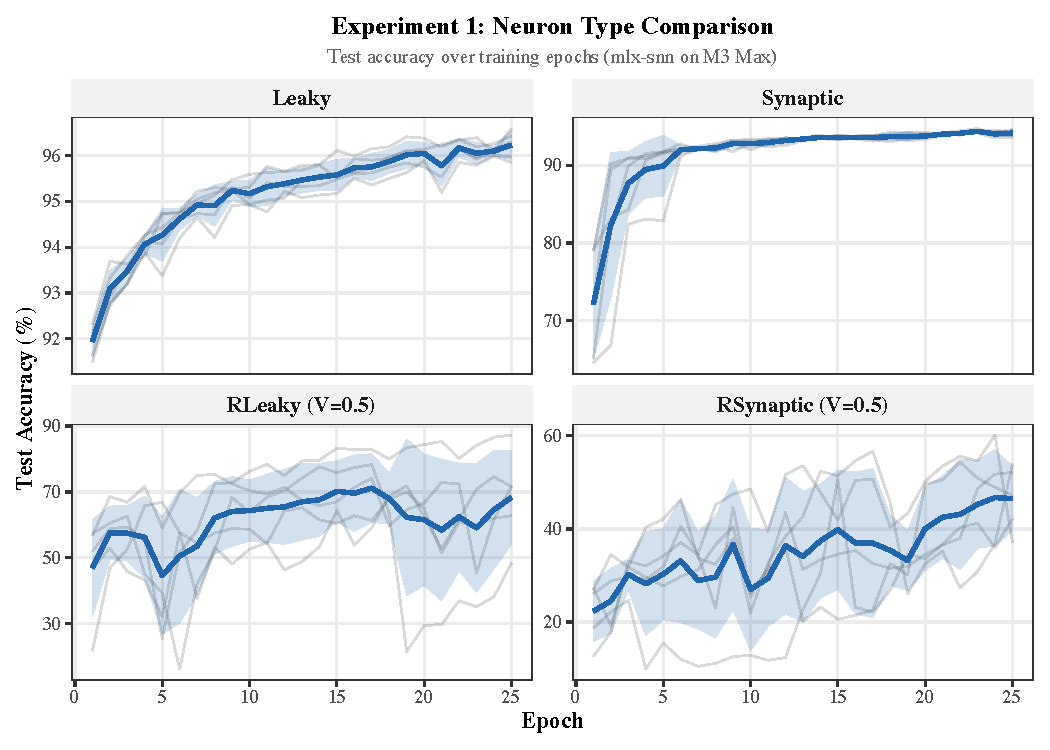
\includegraphics[width=\textwidth]{../figures/fig_learning_curves_exp1.pdf}
\caption{Experiment 1: Learning curves for all neuron types on mlx-snn. Solid lines show mean accuracy over 5 seeds; shaded regions indicate $\pm 1$ standard deviation. Recurrent neurons (RLeaky, RSynaptic) exhibit high variance and slower convergence compared to feedforward counterparts.}
\label{fig:learning_curves_exp1}
\end{figure}

\subsection{Experiment 2: Learnable Parameter Ablation}

Table~\ref{tab:exp2} shows the effect of making $\beta$ and/or the threshold learnable.

\begin{table}[t]
\centering
\caption{Experiment 2: Learnable parameter ablation on MNIST with Leaky neuron. Mean best test accuracy (\%) over 5 seeds (mlx-snn) or 3 seeds (snnTorch).}
\label{tab:exp2}
\small
\begin{tabular}{lcc}
\toprule
\textbf{Configuration} & \textbf{mlx-snn (M3 Max)} & \textbf{snnTorch (V100)} \\
\midrule
Baseline (fixed $\beta$, fixed $V_{\text{thr}}$) & $96.29 \pm 0.24$ & $97.38 \pm 0.09$ \\
\texttt{learn\_beta} & $95.50 \pm 0.33$ & $97.06 \pm 0.08$ \\
\texttt{learn\_threshold} & $96.48 \pm 0.05$ & $97.35 \pm 0.03$ \\
\texttt{learn\_beta} + \texttt{learn\_threshold} & $94.70 \pm 0.16$ & $97.27 \pm 0.10$ \\
\bottomrule
\end{tabular}
\end{table}

On mlx-snn, making the threshold learnable provides a marginal improvement ($96.48\%$ vs.\ $96.29\%$), while learning $\beta$ slightly degrades performance ($95.50\%$). Combining both learnable parameters yields the worst result ($94.70\%$), suggesting optimization interference when both time constants and threshold are jointly adapted on this small architecture.

On snnTorch, all learnable configurations perform within $0.4$ percentage points of the baseline, indicating that the V100 optimizer converges robustly regardless of learnable parameter configuration. The larger gap on mlx-snn ($1.78$ points between best and worst) may reflect differences in the STE-based gradient computation, where the additional learnable parameters introduce gradient paths that interact with the stop-gradient pattern.

\subsection{Experiment 3: Surrogate Gradient Analysis}

Table~\ref{tab:exp3} compares all five surrogate gradient functions.

\begin{table}[t]
\centering
\caption{Experiment 3: Surrogate gradient comparison on MNIST with Leaky neuron. All surrogates use their default scale parameter except where noted.}
\label{tab:exp3}
\small
\begin{tabular}{lcc}
\toprule
\textbf{Surrogate Function} & \textbf{mlx-snn (M3 Max)} & \textbf{snnTorch (V100)} \\
\midrule
Fast Sigmoid ($k=25$) & $96.29 \pm 0.24$ & $96.82 \pm 0.08$ \\
Arctan ($\alpha=2$) & $95.96 \pm 0.17$ & $\mathbf{97.38 \pm 0.09}$ \\
Sigmoid ($k=25$) & $44.82 \pm 13.55$ & $9.91 \pm 0.16$ \\
Triangular & $85.95 \pm 9.51$ & $72.73 \pm 7.02$ \\
Straight-Through & $68.03 \pm 0.92$ & $69.32 \pm 0.82$ \\
\bottomrule
\end{tabular}
\end{table}

Fast sigmoid and arctan are the most effective surrogates on both platforms, consistent with the robustness findings of \citet{zenke2021remarkable}. The standard sigmoid at $k=25$ fails on both platforms ($44.82\%$ on mlx-snn, $9.91\%$ on snnTorch), because the gradient is concentrated in an extremely narrow region around zero, causing vanishing gradients for most neurons.

The triangular surrogate shows a notable cross-platform difference. mlx-snn's tent function achieves $85.95\%$, outperforming snnTorch's sign-flipping implementation ($72.73\%$). This is because snnTorch's triangular gradient assigns $+1$ below threshold and $-1$ above, creating conflicting gradient signals that destabilize training. Our tent function (Eq.~\ref{eq:triangular}) provides a positive, localized gradient that monotonically decays from the threshold, resulting in more stable optimization. Both implementations show high variance ($\pm 9.51\%$ for mlx-snn, $\pm 7.02\%$ for snnTorch), indicating sensitivity to weight initialization. Figure~\ref{fig:learning_curves_exp3} shows the convergence behavior, and Figure~\ref{fig:surrogate_gradients} visualizes the gradient shapes.

The straight-through estimator achieves $68.03\%$ on mlx-snn and $69.32\%$ on snnTorch, showing remarkable cross-platform agreement. Its unbounded gradient (constant 1 everywhere) provides signal to all neurons but lacks the locality that makes fast sigmoid and arctan effective.

\begin{figure}[t]
\centering
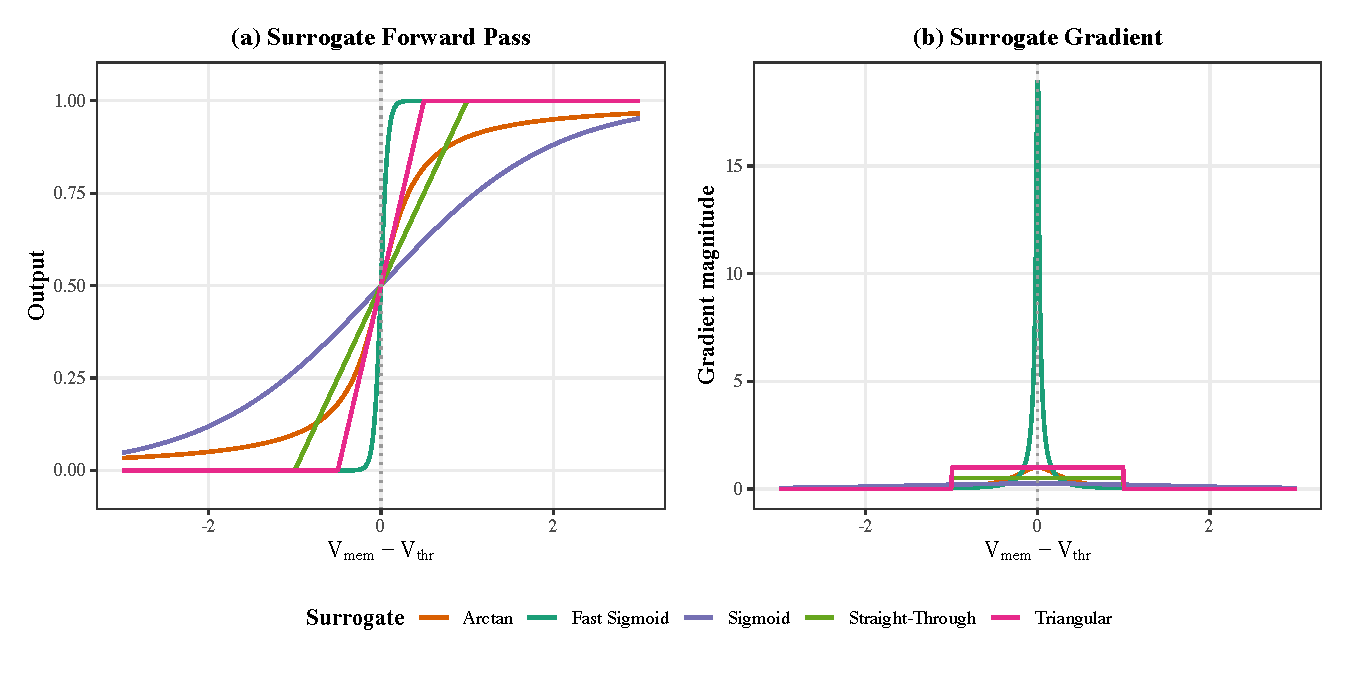
\includegraphics[width=\textwidth]{../figures/fig_surrogate_gradients.pdf}
\caption{Surrogate gradient function shapes. Top row: forward pass (all produce the Heaviside step function). Bottom row: backward pass (smooth surrogate gradients). Note the different scales: sigmoid ($k=25$) has an extremely narrow gradient peak, while straight-through has constant gradient everywhere.}
\label{fig:surrogate_gradients}
\end{figure}

\begin{figure}[t]
\centering
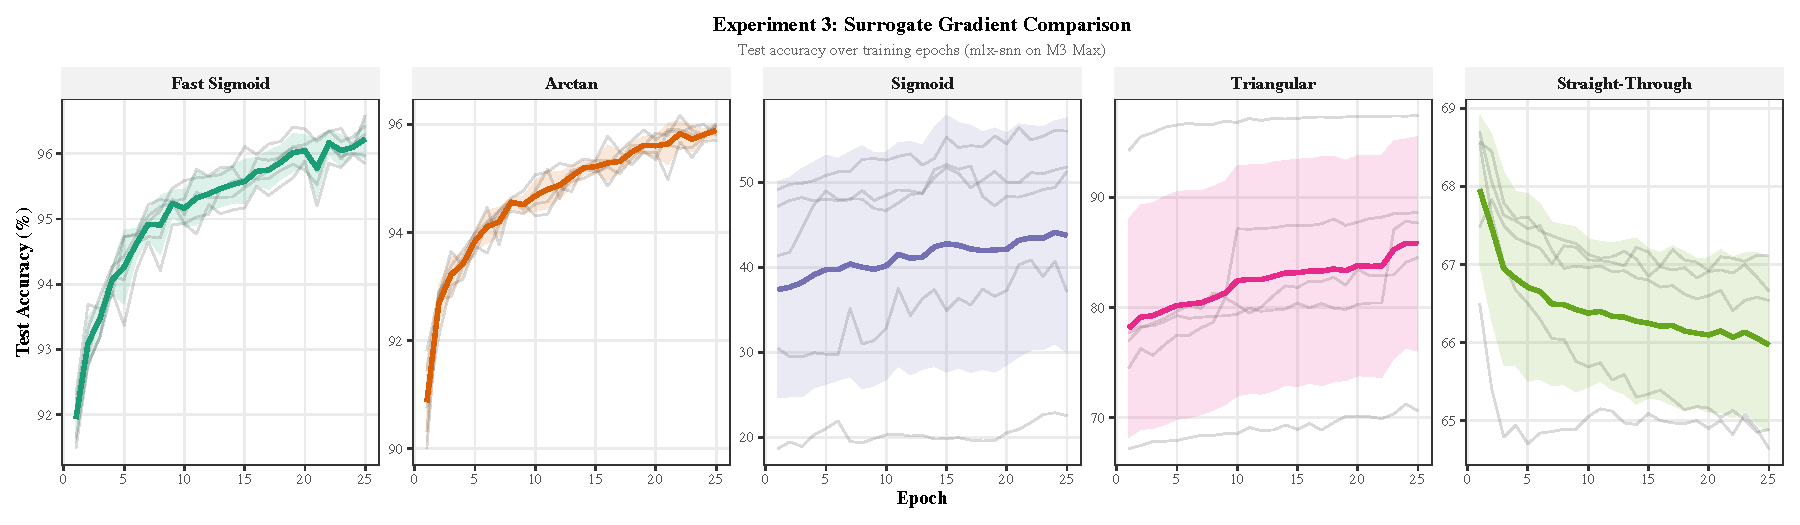
\includegraphics[width=\textwidth]{../figures/fig_learning_curves_exp3.pdf}
\caption{Experiment 3: Learning curves for different surrogate gradient functions on mlx-snn. Fast sigmoid and arctan converge quickly; sigmoid fails to learn; triangular tent and straight-through show intermediate performance.}
\label{fig:learning_curves_exp3}
\end{figure}

\subsection{Experiment 4: Loss Function Comparison}

Table~\ref{tab:exp4} compares the three loss functions.

\begin{table}[t]
\centering
\caption{Experiment 4: Loss function comparison on MNIST with Leaky neuron.}
\label{tab:exp4}
\small
\begin{tabular}{lcc}
\toprule
\textbf{Loss Function} & \textbf{mlx-snn (M3 Max)} & \textbf{snnTorch (V100)} \\
\midrule
CE-Rate (Eq.~\ref{eq:ce_rate}) & $\mathbf{96.29 \pm 0.24}$ & $\mathbf{97.38 \pm 0.09}$ \\
CE-Count (Eq.~\ref{eq:ce_count}) & $93.73 \pm 1.46$ & $97.57 \pm 0.12$ \\
MSE-Membrane (Eq.~\ref{eq:mse_mem}) & $93.12 \pm 0.25$ & $96.99 \pm 0.11$ \\
\bottomrule
\end{tabular}
\end{table}

CE-Rate is the best-performing loss on mlx-snn. On mlx-snn, CE-Count and MSE-Membrane lag by $\sim$2.5--3 percentage points. On snnTorch, CE-Count slightly outperforms CE-Rate ($97.57\%$ vs.\ $97.38\%$), while MSE-Membrane shows a slight degradation ($96.99\%$).

The gap on mlx-snn for CE-Count is notable because CE-Rate and CE-Count differ only in whether the temporal sum is divided by $T$. This normalization appears to stabilize gradient magnitudes when combined with the STE surrogate pattern. Without normalization (CE-Count), the logits grow proportionally with $T$, potentially saturating the softmax and reducing gradient effectiveness. CE-Count also shows higher variance ($\pm 1.46\%$) compared to CE-Rate ($\pm 0.24\%$).

MSE-Membrane loss, which uses only the final timestep's membrane potential rather than aggregating over time, discards temporal information and is more sensitive to the specific trajectory of the membrane potential during the last few timesteps.

\subsection{Experiment 5: Encoding Strategy Comparison}

Table~\ref{tab:exp5} compares the three encoding strategies.

\begin{table}[t]
\centering
\caption{Experiment 5: Encoding strategy comparison on MNIST with Leaky neuron.}
\label{tab:exp5}
\small
\begin{tabular}{lcc}
\toprule
\textbf{Encoding} & \textbf{mlx-snn (M3 Max)} & \textbf{snnTorch (V100)} \\
\midrule
Rate (Poisson) & $\mathbf{96.29 \pm 0.24}$ & $\mathbf{97.38 \pm 0.09}$ \\
Latency (TTFS) & $89.33 \pm 8.44$ & $94.48 \pm 0.04$ \\
Delta & $46.47 \pm 1.10$ & $82.45 \pm 0.17$ \\
\bottomrule
\end{tabular}
\end{table}

Rate coding achieves the best accuracy on both platforms. Latency coding shows a $\sim$7 point degradation on average ($89.33\%$), but with very high variance ($\pm 8.44\%$), indicating that time-to-first-spike encoding is sensitive to random initialization. Some seeds achieve $>$95\% while others fall below 80\%.

Delta modulation performs poorly on both platforms, particularly on mlx-snn ($46.47\%$). This encoding is fundamentally mismatched with static MNIST images: delta encoding computes temporal differences, but MNIST images are presented as constant inputs across all timesteps, resulting in zero spikes after the first timestep (or throughout, depending on the padding convention). The higher snnTorch accuracy ($82.45\%$) on delta encoding suggests potential differences in the encoding implementation (e.g., how the first timestep is handled) that partially compensate for this mismatch.

\subsection{Cross-Platform Performance Analysis}

Figure~\ref{fig:training_speed} and Table~\ref{tab:speed} summarize the training speed comparison across both platforms.

\begin{table}[t]
\centering
\caption{Training speed comparison: mlx-snn on Apple M3 Max vs.\ snnTorch on NVIDIA V100. Seconds per epoch on MNIST with batch size 128.}
\label{tab:speed}
\small
\begin{tabular}{lccc}
\toprule
\textbf{Neuron} & \textbf{mlx-snn (M3 Max)} & \textbf{snnTorch (V100)} & \textbf{Speedup} \\
\midrule
Leaky & 5.7 & 20.9 & $3.7\times$ \\
RLeaky & 6.4 & 25.8 & $4.0\times$ \\
Synaptic & 6.1 & 25.2 & $4.1\times$ \\
\bottomrule
\end{tabular}
\end{table}

mlx-snn on the M3~Max is $3.7\times$ faster per epoch than snnTorch on the V100 for the baseline Leaky neuron. Recurrent and synaptic neurons are marginally slower due to additional state variables and computations but remain well under 7\,s/ep. This speed advantage stems from MLX's unified memory architecture (zero-copy data access between CPU and GPU), lazy evaluation (whole-graph optimization before execution), and the relatively small model size that fits entirely in the M3~Max's large unified memory without memory pressure.

\begin{figure}[t]
\centering
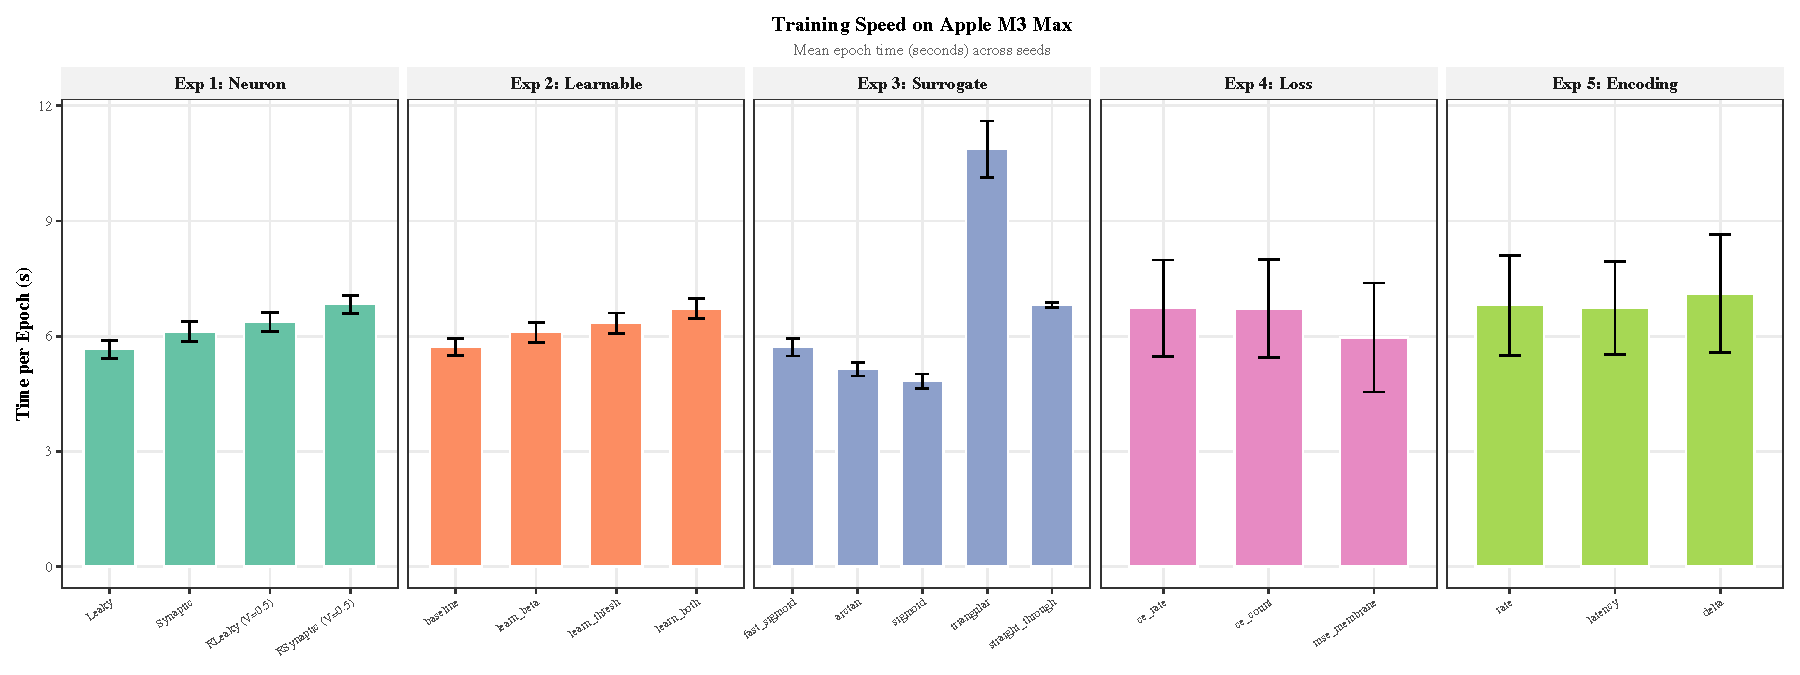
\includegraphics[width=0.9\textwidth]{../figures/fig_training_speed.pdf}
\caption{Training speed comparison across neuron types. mlx-snn on Apple M3 Max (blue) vs.\ snnTorch on NVIDIA V100 (orange). Error bars indicate standard deviation across seeds.}
\label{fig:training_speed}
\end{figure}

\subsection{Summary Across All Experiments}

Figure~\ref{fig:heatmap_all_results} provides a comprehensive heatmap view of accuracy across all experimental conditions.

\begin{figure}[t]
\centering
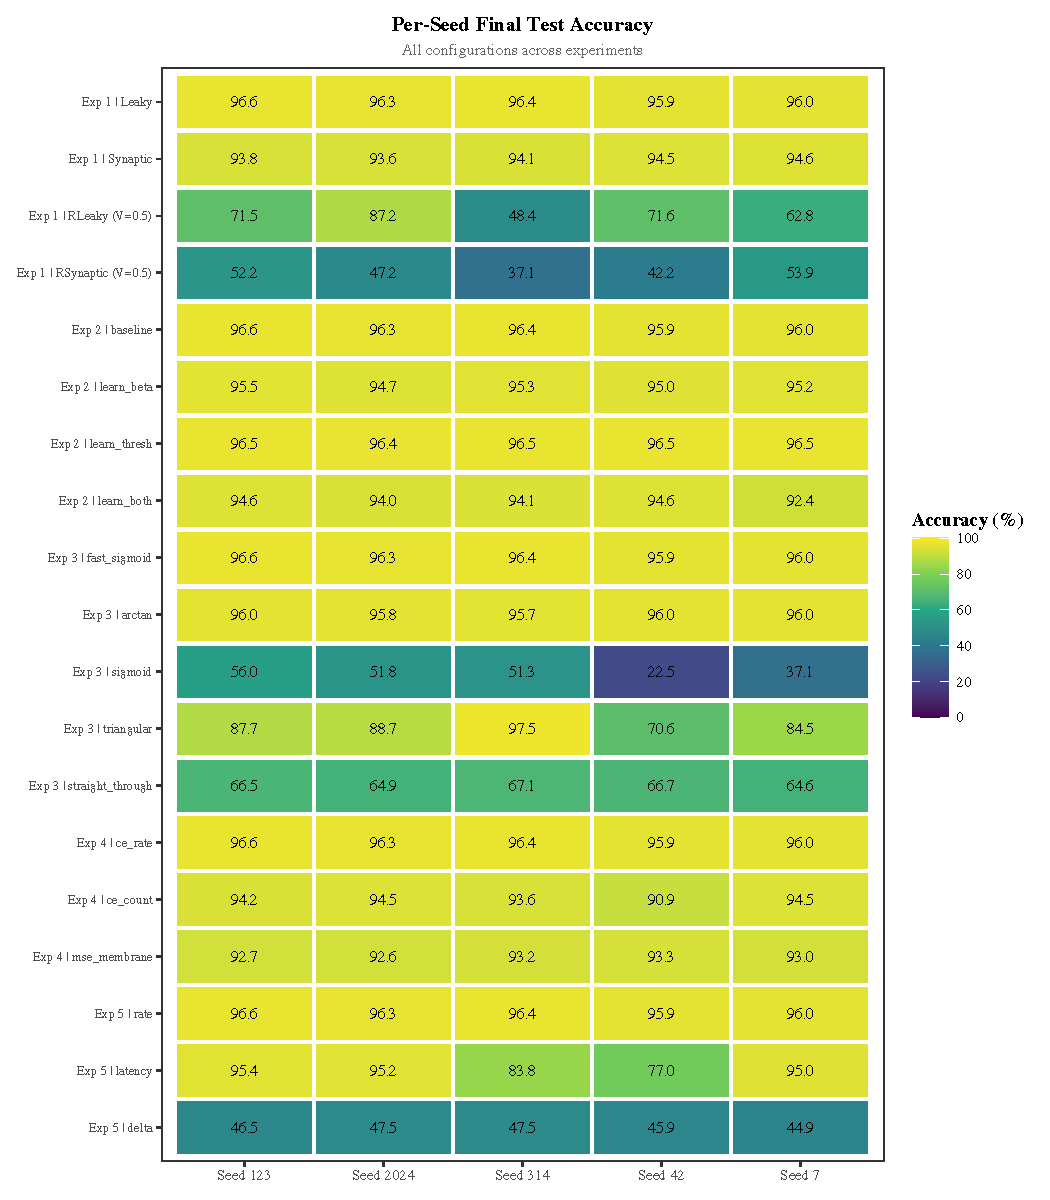
\includegraphics[width=\textwidth]{../figures/fig_heatmap_all_results.pdf}
\caption{Heatmap of test accuracy (\%) across all experimental conditions for mlx-snn (M3 Max) and snnTorch (V100). Darker colors indicate higher accuracy. The consistent $1$--$2\%$ gap between platforms is visible across most configurations, with larger divergences for recurrent neurons and delta encoding.}
\label{fig:heatmap_all_results}
\end{figure}

\begin{figure}[t]
\centering
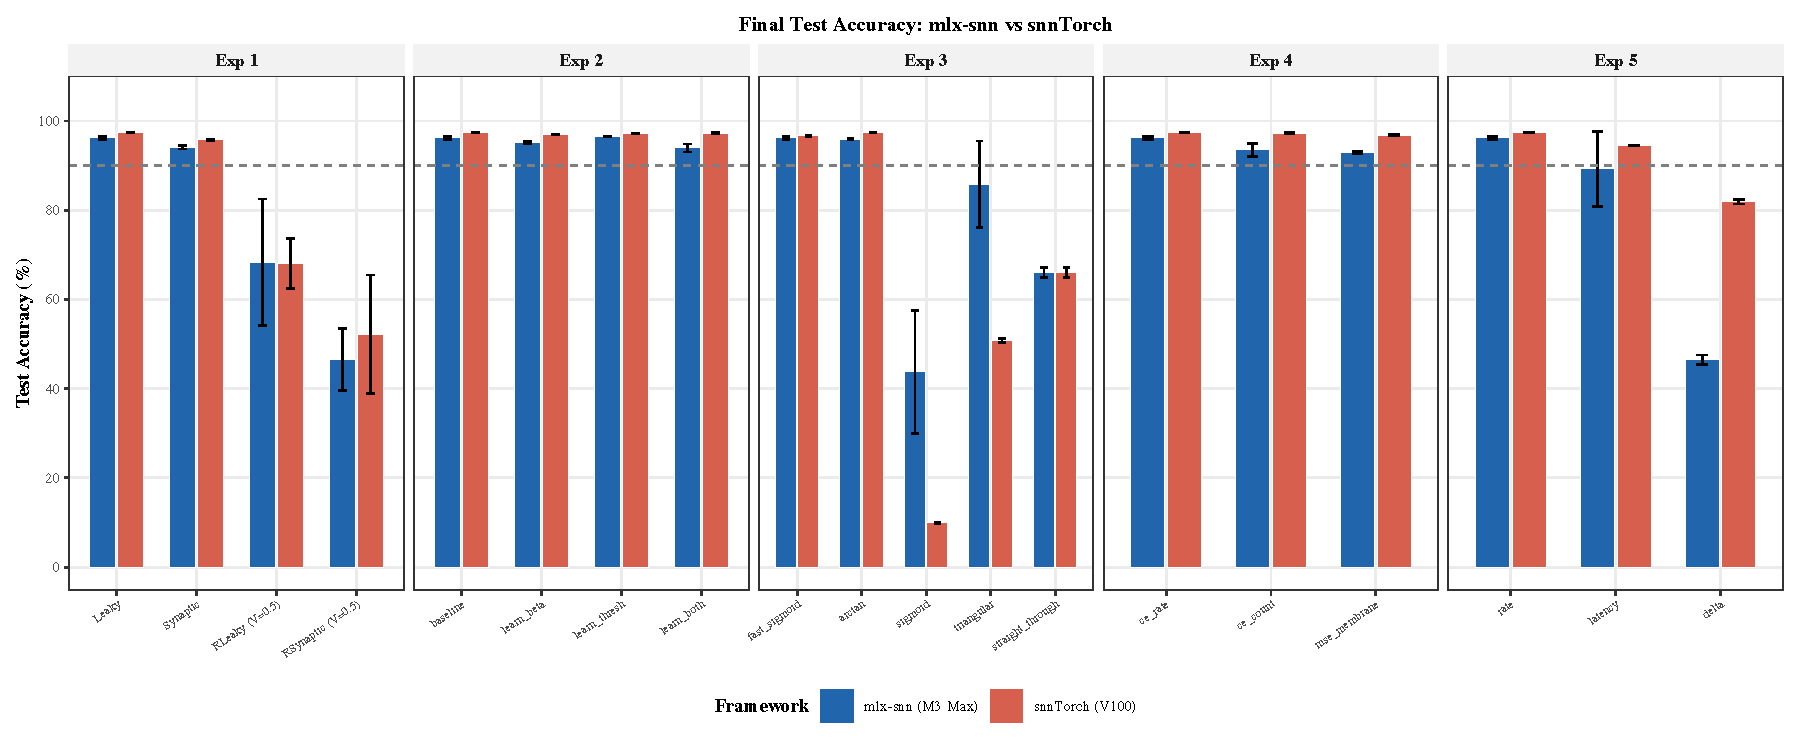
\includegraphics[width=\textwidth]{../figures/fig_accuracy_comparison.pdf}
\caption{Side-by-side accuracy comparison across all five experiments. mlx-snn (blue) vs.\ snnTorch (orange). Error bars show $\pm 1$ standard deviation.}
\label{fig:accuracy_comparison}
\end{figure}

% ===================================================================
% 6. DISCUSSION
% ===================================================================
\section{Discussion}

\subsection{Key Findings}

Our benchmarking study reveals several important findings for the SNN research community:

\paragraph{Feedforward neurons dominate on MNIST.}
The standard LIF neuron achieves the best accuracy on both platforms, outperforming more complex recurrent and synaptic variants. This is not surprising for the relatively simple MNIST task, where temporal dynamics beyond basic membrane decay add complexity without proportional representational benefit. The Synaptic neuron's two-state dynamics provide marginal smoothing at minimal accuracy cost, while recurrent neurons require careful initialization to avoid instability.

\paragraph{Recurrent weight initialization is critical.}
The recurrent weight $V$ in RLeaky and RSynaptic neurons has an outsized effect on training dynamics. Values of $V \geq 0.5$ cause the recurrent feedback to dominate the membrane dynamics, leading to either persistent firing (all neurons spike every timestep) or complete silencing (no neurons spike), depending on the interplay with the reset mechanism. Reducing $V$ to $0.1$ and making it learnable substantially improves results, but variance remains high. This sensitivity is consistent across platforms and represents a fundamental challenge of recurrent SNN design, not a framework artifact.

Figure~\ref{fig:recurrent_V_comparison} illustrates the learning curve divergence between different $V$ initializations.

\begin{figure}[t]
\centering
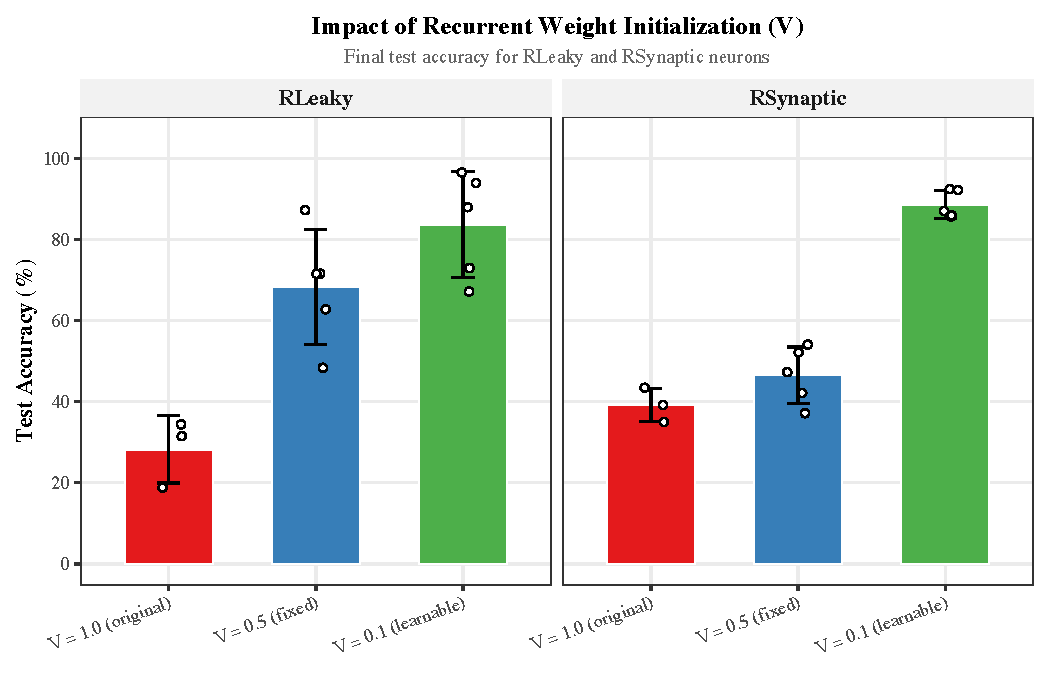
\includegraphics[width=0.9\textwidth]{../figures/fig_recurrent_V_comparison.pdf}
\caption{Effect of recurrent weight $V$ initialization on RLeaky and RSynaptic convergence. Lower $V$ initialization with learnable $V$ produces more stable but still high-variance training.}
\label{fig:recurrent_V_comparison}
\end{figure}

\paragraph{Surrogate gradient implementation matters more than function choice.}
While \citet{zenke2021remarkable} found that network performance is robust to surrogate function choice, our results show that \emph{implementation details} can cause large performance differences. The triangular surrogate exemplifies this: mlx-snn's tent function achieves $85.95\%$ while snnTorch's sign-flipping variant reaches only $72.73\%$. Both are valid interpretations of a ``triangular'' surrogate, but the tent function's positive, localized gradient is substantially more effective for gradient-based optimization. Similarly, the standard sigmoid at scale $k=25$ fails catastrophically on both platforms due to its extremely narrow gradient peak --- a consequence of the default hyperparameter rather than the function itself.

\paragraph{Cross-entropy on rate is the most robust loss.}
CE-Rate consistently outperforms CE-Count and MSE-Membrane across both platforms. The temporal averaging in CE-Rate implicitly normalizes gradient magnitudes, preventing the logit scale from growing with $T$. This is particularly important for SNN training where the number of timesteps directly affects the scale of spike counts.

\subsection{Cross-Platform Analysis}

\paragraph{Speed vs.\ accuracy trade-off.}
mlx-snn on the M3~Max achieves $3.7$--$4.1\times$ faster training than snnTorch on the V100, with a consistent $\sim$1 percentage point accuracy gap. This gap is attributable to the STE-based surrogate gradient pattern (Eq.~\ref{eq:ste}), which is necessitated by MLX's current limitations with custom VJP definitions. The STE pattern provides correct Heaviside forward behavior and smooth gradients, but the gradient path through \texttt{mx.stop\_gradient} differs subtly from a native custom backward pass, particularly in how gradient magnitudes are scaled during backpropagation through time. We expect this gap to narrow as MLX's \texttt{mx.custom\_function} API matures.

\paragraph{Unified memory advantage.}
The M3~Max's 128\,GB unified memory means that CPU preprocessing (data loading, augmentation) and GPU computation (forward/backward passes) share the same physical memory, eliminating the PCIe transfer overhead that exists between CPU RAM and V100 HBM2. For the relatively small MNIST workload, this architectural advantage significantly reduces per-epoch overhead. Larger models and datasets may see different trade-offs as compute intensity grows relative to memory transfer costs.

\paragraph{Hardware generational context.}
The NVIDIA V100 (released 2017, Volta architecture) is now an older-generation GPU. A more contemporary comparison against an A100 or H100 would likely narrow the speed gap. However, the V100 remains widely available in academic computing clusters and cloud instances, making it a relevant reference point for the research community. The key takeaway is that Apple Silicon provides competitive SNN training performance without requiring dedicated GPU infrastructure.

\subsection{Limitations}

\paragraph{Dataset scope.}
All experiments use MNIST, a small and relatively simple benchmark. Performance rankings and hyperparameter sensitivities may differ on more challenging neuromorphic datasets (N-MNIST, SHD, DVS-Gesture) or larger-scale tasks (CIFAR-10, ImageNet). Extending our benchmark suite to these datasets is a priority for future work.

\paragraph{Architecture scale.}
The $784$--$128$--$10$ architecture is deliberately small to enable comprehensive sweeps with multiple seeds. Convolutional SNNs, deeper architectures, and larger hidden dimensions may exhibit different trade-offs between neuron types, surrogate functions, and platforms.

\paragraph{snnTorch seed count.}
Due to limited V100 access, snnTorch experiments use 3 seeds compared to mlx-snn's 5 seeds. This provides less statistical power for snnTorch results, particularly for high-variance conditions (recurrent neurons).

\paragraph{Recurrent neuron configurations.}
The snnTorch recurrent neuron experiments use $V=1.0$ (learnable) while mlx-snn uses $V=0.1$ and $V=0.5$, making direct comparison of RLeaky and RSynaptic across platforms imperfect. However, both platforms demonstrate the same qualitative sensitivity to $V$ initialization.

% ===================================================================
% 7. PRACTICAL GUIDELINES
% ===================================================================
\section{Practical Guidelines for SNN Training on Apple Silicon}

Based on our experimental findings, we offer the following recommendations for practitioners:

\begin{enumerate}[leftmargin=*]
    \item \textbf{Start with Leaky/LIF.} The standard LIF neuron provides the best accuracy-to-complexity ratio. Use $\beta = 0.9$ as a default starting point.

    \item \textbf{Use fast sigmoid or arctan surrogates.} These two functions provide robust gradient signal across a wide range of membrane potentials. Avoid the standard sigmoid at the default scale ($k=25$); if sigmoid is desired, reduce the scale to $k \leq 5$.

    \item \textbf{Prefer CE-Rate loss.} The temporal averaging normalizes gradient magnitudes and provides the most stable training. CE-Count can work but may require learning rate adjustment.

    \item \textbf{Initialize recurrent weights small.} If using RLeaky or RSynaptic, initialize $V \leq 0.1$ and make it learnable. Values of $V \geq 0.5$ frequently cause training collapse.

    \item \textbf{Use rate encoding for static data.} Rate coding is the most forgiving encoding for image classification. Reserve latency encoding for applications where temporal precision matters, and delta encoding for truly temporal (time-varying) signals.

    \item \textbf{Keep threshold fixed.} Making the threshold learnable provides marginal benefit and can destabilize training when combined with learnable $\beta$. If adaptation is needed, learn either $\beta$ or threshold, not both.

    \item \textbf{Leverage unified memory.} Batch sizes of 128--256 work well on M3~Max. The unified memory architecture means that increasing batch size does not incur CPU--GPU transfer penalties, so larger batches are cost-effective for throughput.
\end{enumerate}

% ===================================================================
% 8. CONCLUSION
% ===================================================================
\section{Conclusion}

We have presented a comprehensive benchmarking study of spiking neural network training using mlx-snn v0.4 on Apple Silicon. Through five systematic experiments on MNIST with multiple random seeds, we have evaluated the effects of neuron type, learnable parameters, surrogate gradient function, loss function, and spike encoding strategy. Our cross-platform comparison between mlx-snn on an Apple M3~Max and snnTorch on an NVIDIA V100 reveals that Apple Silicon provides $3.7$--$4.1\times$ faster training with competitive accuracy, establishing mlx-snn as a viable alternative for SNN research without dedicated GPU infrastructure.

Key findings include the critical sensitivity of recurrent neurons to weight initialization, the superiority of the triangular tent surrogate over sign-flipping implementations, and the robustness of cross-entropy on spike rate as a loss function. These results provide actionable guidelines for SNN practitioners on Apple Silicon and motivate further development of the mlx-snn ecosystem.

mlx-snn v0.4 is available on PyPI (\texttt{pip install mlx-snn}) and GitHub under the MIT license. Future work includes extending benchmarks to neuromorphic datasets (SHD, N-MNIST, DVS-Gesture), implementing convolutional SNN layers, adding liquid state machine support, and developing \texttt{mx.compile}-optimized training loops as MLX continues to mature.

\bigskip
\noindent\textbf{Reproducibility.} All experiment scripts, configuration files, and analysis notebooks are available in the project repository at \url{https://github.com/D-ST-Sword/mlx-snn/tree/main/experiments}.

\bigskip
\noindent\textbf{Citation.}
\begin{verbatim}
@article{qin2026mlxsnn_v2,
  title   = {Comprehensive Benchmarking of Spiking Neural
             Networks on Apple Silicon: mlx-snn v0.4},
  author  = {Qin, Jiahao},
  journal = {arXiv preprint arXiv:XXXX.XXXXX},
  year    = {2026}
}
\end{verbatim}

% ===================================================================
% REFERENCES
% ===================================================================
\bibliographystyle{plainnat}
\bibliography{references}

\end{document}
